\documentclass[11pt]{article}
\usepackage[]{amsfonts, amssymb, amsmath, float, hyperref,fancyheadings, graphicx, derivative}
\usepackage[utf8]{inputenc}
\usepackage{pgfplots}
\pgfplotsset{compat=1.18, width=8cm}
\usepackage{geometry}
\geometry{
a4paper,
total={170mm,257mm},
left=20mm,
top=20mm,
}
\title{Making plots in \latex}
\author{Larry}
\date{Aug 2024}
\begin{document}

\tableofcontents
\section{2D plots}
\begin{tabular}{cc}
\begin{tikzpicture}
\begin{axis}[xmin=-2, xmax=2, ymin=-2, ymax=2, 
axis lines= middle, 
xlabel= $x$, 
ylabel= $y$,
title = {2D plot Sample 1}]

\addplot[color = red, dashed, samples = 100, domain = -1: 1]{x^2};
\addplot[color = blue, dotted, samples = 100]{1- x^2};

\end{axis}
\end{tikzpicture}&
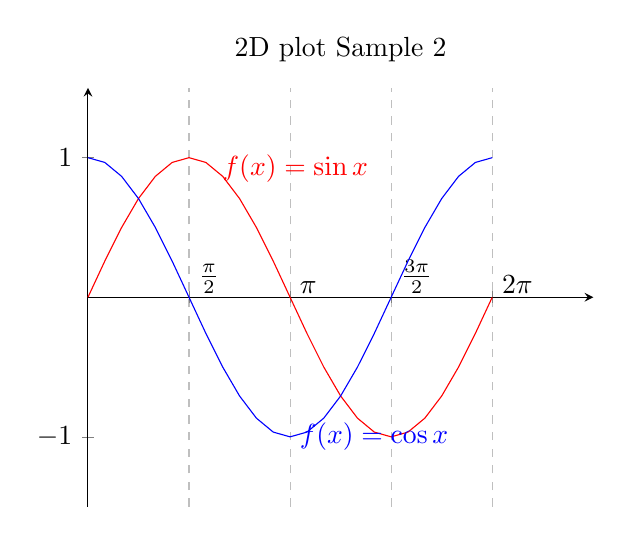
\begin{tikzpicture}

\begin{axis}[clip = false,
axis lines= middle,
xmin = 0,
xmax = 2.5*pi,
ymin= -1.5,
ymax = 1.5,
title = {2D plot Sample 2},
xtick = {0, pi/2, pi, 1.5*pi, 2*pi},
xticklabels={$0$, $\frac{\pi}{2}$,$\pi$, $\frac{3\pi}{2}$, $2\pi$},
xticklabel style = {anchor= south west},
xmajorgrids = true,
grid style = dashed]

\addplot[domain= 0:2*pi, color = red]{sin(deg(x))}{node[right, pos=0.3]{$f(x) = \sin x$}};
\addplot[domain= 0:2*pi, color = blue]{cos(deg(x))}{node[right, pos=0.5]{$f(x) = \cos x$}};

\end{axis}
\end{tikzpicture}\\

\begin{tikzpicture}
\begin{axis}[
title= {Scatter plot of GPA versus Ages},
xlabel = $GPA$, 
ylabel = $Ages$]
\addplot+[
only marks,
scatter,
mark size= 1.5 pt]
table[meta= Ages]{test.txt};
\end{axis}
\end{tikzpicture}&

\begin{tikzpicture}
\begin{axis}[
title= {Scatter plot of GPA versus Wages},
xlabel = $GPA$, 
ylabel = $Wages$]
\addplot+[
only marks,
scatter,
mark size= 1.5 pt]
table[meta= Wages]{test.txt};
\end{axis}
\end{tikzpicture}\\

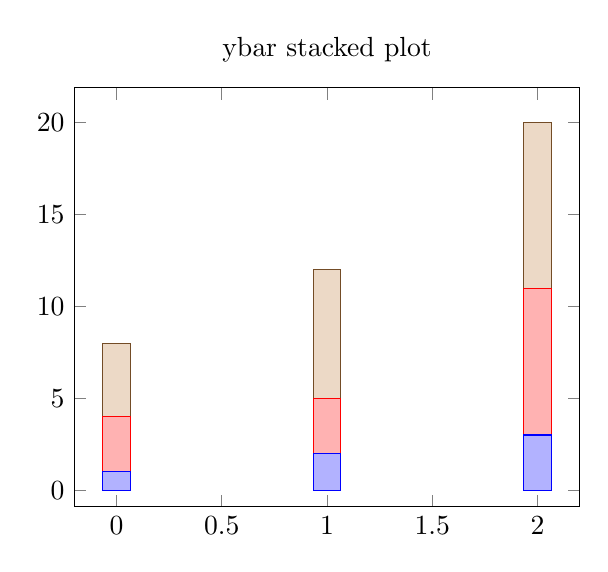
\begin{tikzpicture}

\begin{axis}[ybar stacked, title = {ybar stacked plot}]
\addplot coordinates
{(0, 1) (1, 2) (2, 3)};
\addplot coordinates
{(0, 3) (1, 3) (2, 8)};
\addplot coordinates
{(0, 4) (1, 7) (2, 9)};
\end{axis}

\end{tikzpicture}

\end{tabular}

\section{3D plots}
\begin{tabular}{cc}

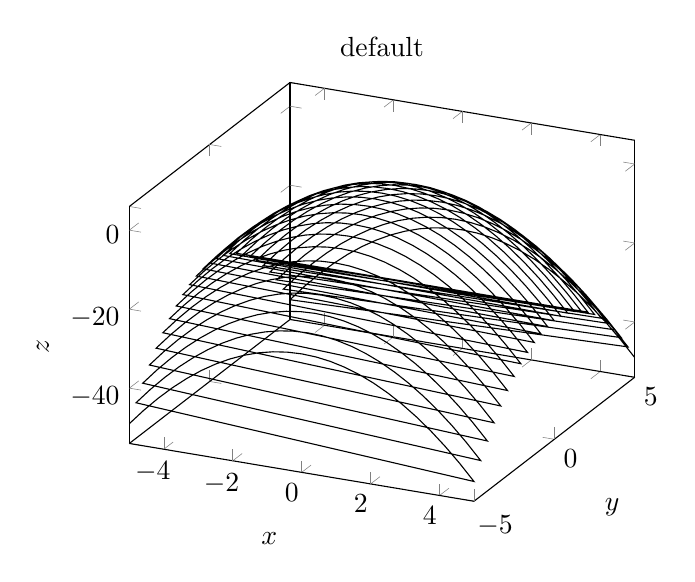
\begin{tikzpicture}
\begin{axis}[title= {default},
xlabel = $x$,
ylabel = $y$,
zlabel = $z$]
\addplot3 [] {1- x^2 - y^2};
\end{axis}
\end{tikzpicture}&

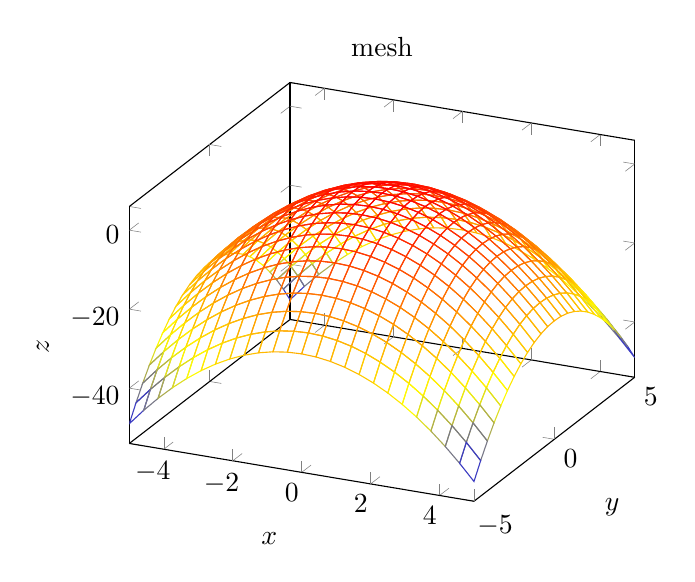
\begin{tikzpicture}
\begin{axis}[title = {mesh},
xlabel = $x$,
ylabel = $y$,
zlabel = $z$]
\addplot3 [mesh] {1- x^2 - y^2};
\end{axis}
\end{tikzpicture}\\

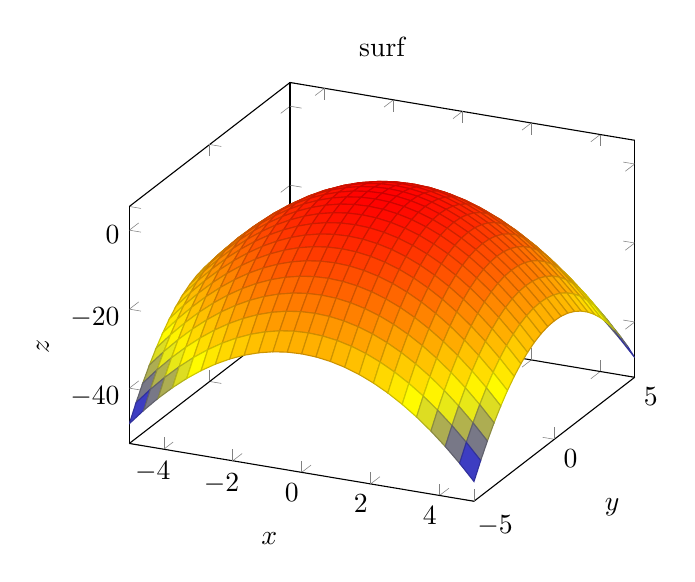
\begin{tikzpicture}
\begin{axis}[title= {surf},
xlabel = $x$,
ylabel = $y$,
zlabel = $z$]
\addplot3 [surf] {1- x^2 - y^2};
\end{axis}
\end{tikzpicture}&

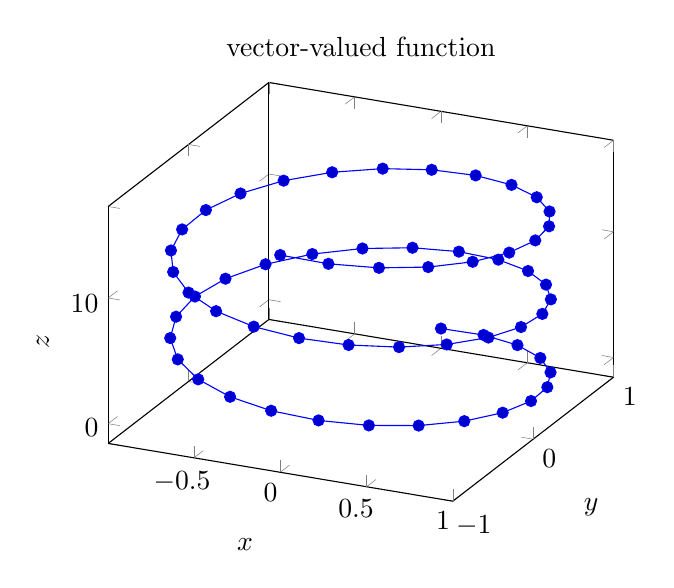
\begin{tikzpicture}
\begin{axis}[title= {vector-valued function},
xlabel = $x$,
ylabel = $y$,
zlabel = $z$]
\addplot3+[domain= 0:5*pi, samples= 60, samples y= 0]
({sin(deg(x))},
{cos(deg(x))},
{x});
\end{axis}
\end{tikzpicture}\\

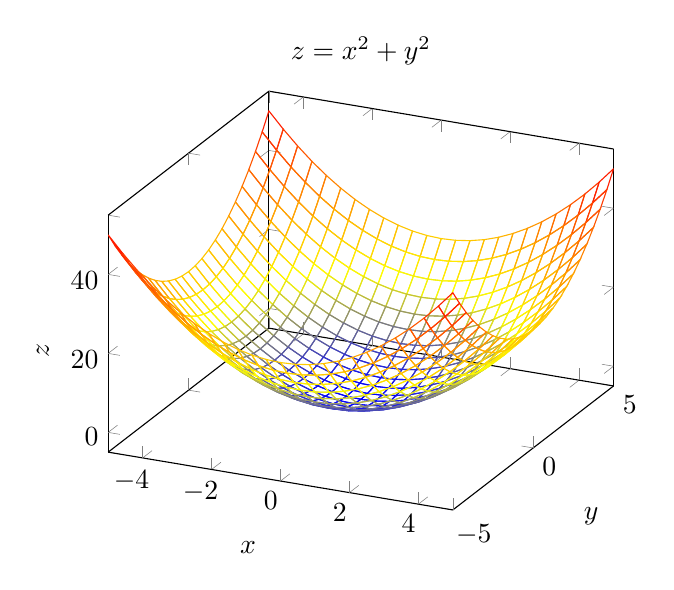
\begin{tikzpicture}
\begin{axis} [title = {$z = x^2 + y^2$},
xlabel = $x$,
ylabel = $y$,
zlabel = $z$
]
\addplot3 [mesh]{x^2 + y^2};
\end{axis}
\end{tikzpicture}&

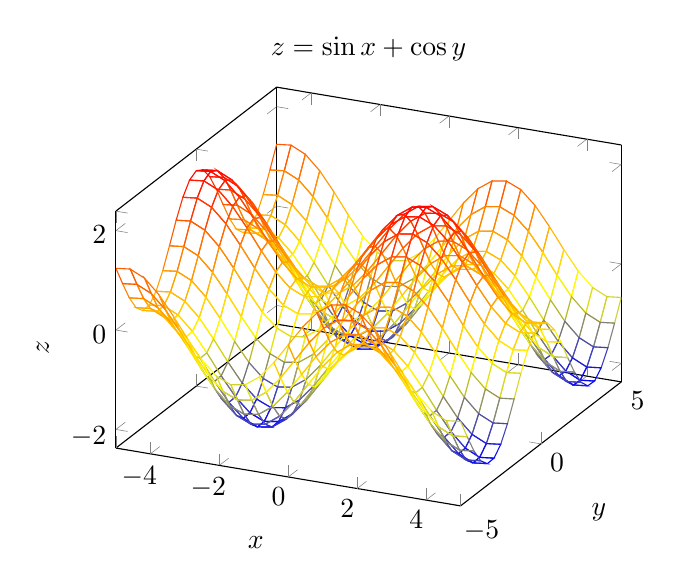
\begin{tikzpicture}
\begin{axis} [title = {$z = \sin x + \cos y$},
xlabel = $x$,
ylabel = $y$,
zlabel = $z$
]
\addplot3 [mesh]{sin(deg(x)) + cos(deg(y))};
\end{axis}
\end{tikzpicture}
\end{tabular}

\section{vectors}
\begin{tabular}{cc}
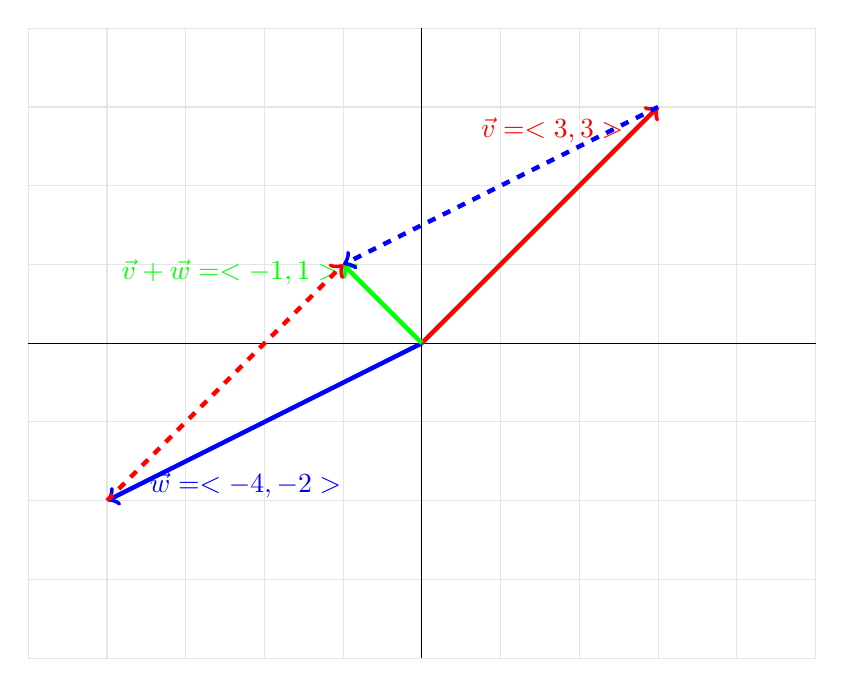
\begin{tikzpicture}[scale = 1]
\draw[thin,gray!20] (-5,-4) grid (5, 4);
\draw (5, 0) -- (-5, 0) (0, 4) -- (0, -4);
\draw [->, ultra thick, color = red] (0, 0) -- (3,3) {node[left, pos=0.9]{$\vec{v} = <3, 3>$}};
\draw [->, ultra thick, color = blue] (0, 0) -- (-4, -2) {node[right, pos=0.9]{$\vec{w} = <-4, -2>$}};
\draw [->, ultra thick, color = green] (0, 0) -- (-1, 1) {node[left, pos=0.9]{$\vec{v} + \vec{w} = <-1, 1>$}};
\draw [->, ultra thick, color = blue, dashed] (3, 3) -- (-1, 1);
\draw [->, ultra thick, color = red, dashed] (-4, -2) -- (-1, 1);
\end{tikzpicture}&
\begin{tikzpicture}
\draw [-latex] (0, 0, 0) -- (5, 0, 0) node[left]{$x$};
\draw [-latex] (0, 0, 0) -- (0, 5, 0) node[left]{$y$};
\draw [-latex] (0, 0, 0) -- (0, 0, 5) node[left]{$z$};
\draw [->, ultra thick, blue] (0, 0, 0) -- (3, 2, 1) node[pos=0.7, right] {$\vec{a} = <3, 2, 1>$};
\draw [dashed, - , blue] (3, 0, 0) -- (3, 0, 1);
\draw [dashed, - , blue] (0, 0, 1) -- (3, 0, 1);
\draw [dashed, - , blue] (0, 2, 0) -- (3, 2, 1);
\draw [dashed, - , blue] (3, 0, 1) -- (3, 2, 1);
\end{tikzpicture}
\end{tabular}




\end{document}